\@specialtrue
\cxset{steward,
  numbering=arabic,
  custom=stewart,
  offsety=0cm,
  image=hine05,
  texti={When Lamport designed the original \LaTeX\ sectioning commands, limitations of computer power forced him to restrict the abstraction of complicated chapter layouts. With current tools available improvements are much easier to program.},
  textii={In this chapter we discuss a method that allows the production of fancy chapter headings and formatting, based on a set of key values. Central  to this process is the separation of content from presentation.
We also discuss the basic formatting tools that are available and how one can modify them to mould new book designs.
 }
}
\cxset{chapter opening=left}

\chapter{General Settings}

\section{Introduction}

Here we define and set general paragraph settings. The parameters which control \TeX's behaviour when typesetting paragraphs can receive a bit of a tweak here. We also describe a set of options to handle parameters that can influence grid typesetting. This is especially important for two or more column typesetting.

\subsection{Parameters controlling paragraphs}\index{Paragraphs!controlling parameters}
The parameters \cs{lineskip} and \cs{normallineskip} influence \TeX\ when two lines come two close.
\medskip

\keyval{lineskip}{\marg{dim}}{Lineskip parameter}
\keyval{normallineskip}{\marg{dim}}{Lineskip parameter.}
\keyval{lineskiplimit}{\marg{number}}{Lineskip limit}
\keyval{parindent}{\marg{dim}}{Paragraph indentation.}
\keyval{text-indent}{\marg{dim}}{Alias for \cs{parindent}.}
\keyval{parskip}{\marg{dim}}{Spacing between paragraphs.}

\cxset{lineskip/.code=\setlength\lineskip{#1},
          normallineskip/.code=\setlength\normallineskip{#1},
          parindent/.code=\setlength\parindent{#1},
          parskip/.code=\setlength\parskip{#1},
          text-indent/.code=\setlength\parindent{#1},
          baselinestretch/.code=\renewcommand\baselinestretch{#1}}



\begin{texexample}{Paragraph parameters, using CSS style commands}{}{}
\cxset{lineskip=1pt,
          normallineskip=1pt,
          parindent=1em}

\lipsum[1]

\cxset{
          lineskip=2pt,
          normallineskip=2pt,
          parindent=1.5em,
          parskip=3pt,
          baselinestretch={},
 }
\linenottooshort[20em]

\lipsum[1-2]
\lorem

\end{texexample}

These command offer little value over the normal \TeX\ macros other than keeping the interface, uniform. One can also extend the interface to cover CSS style commands:

\begin{texexample}{Paragraph parameters}{}
\cxset{text-indent=50pt}
\vbox to 4cm{\lipsum*[1]}
\end{texexample}

Another advantage, the package offers a few pre-configured styles, just setting a style to latex will revert everything back to latex.

\section{Technical discussion}

Most classes, including the standard \LaTeXe\ classes as well as packages attempting to achieve a grid typesetting try define a text height that is a multiple of \cs{baselineskip}. This way they give little opportunity to TeX to adjust the vertical glue to achieve a flush bottom.

\section{Dropcaps and Lettrines}\index{Lettrine!basic typesetting}

Dropcaps or lettrines are those letters that start paragraphs with a fancy larger letter. The class uses a parameterized version of the lettrine package of Daniel Flipo. Lettrine letters are easily typed and produced, but they are notoriously difficult to get right and no-one seems to agree on settings. These settings depend on the font the sizing of the text and the personal taste of the book interior designer. As I don't profess to be one, I have done what I think Knuth have done (just studied existing sources) allowed programming hooks and provided defaults as close as possible to the originals.


\subsection{Grid typesetting}
\the\textheight

\begin{tcolorbox}{title= Grid type typesetting}
%\begin{lstlisting}
\def\Grid@baseline{10\p@}
\def\Grid@fontsize{12\p@}
\def\Grid@lines{40}
\def\Grid@textheight{%
       \@tempdima=\Grid@baseline%
       \multiply\@tempdima by \Grid@lines%
       \textheight=\the\@tempdima%
}
\Grid@textheight
\renewcommand\normalsize{%
   \baselineskip=\Grid@baseline%
   \@setfontsize\normalsize{\Grid@fontsize}{\Grid@baseline}%
   \lineskip=0pt
   \lineskiplimit=-\Grid@fontsize%
   \abovedisplayskip \baselineskip%
   \abovedisplayshortskip .5\baselineskip%
   \belowdisplayskip \abovedisplayskip
   \belowdisplayshortskip \abovedisplayshortskip
   \let\@listi\@listI}
\normalsize
%\end{lstlisting}
\end{tcolorbox}
\newdimen\floatunit
\newskip\allfloats
\setlength\floatunit{\the\baselineskip}

\setlength\allfloats{\floatunit}

\setlength\floatsep{\allfloats}
\setlength\textfloatsep{\allfloats}
\setlength\intextsep{\allfloats}
\setlength\dblfloatsep{\allfloats}
\setlength\dbltextfloatsep{\allfloats}

\setlength\@fptop{\z@}
\setlength\@fpsep{\z@}
\setlength\@fpbot{\z@}
\setlength\@dblfptop{\z@}
\setlength\@dblfpsep{\z@}
\setlength\@dblfpbot{\z@}

\begingroup
  \catcode`P=12
  \catcode`T=12
  \lowercase{
    \def\x{\def\rem@decimal##1.##2PT{##1}}}
  \expandafter\endgroup\x
\def\strip@decimal{\expandafter\rem@decimal\the}

\begingroup
  \catcode`P=12
  \catcode`T=12
  \lowercase{
    \def\y{\def\rem@dot##1.##2PT{##1##2}}}
  \expandafter\endgroup\y
\def\strip@dot{\expandafter\rem@dot\the}

\newdimen\halfbaselineskip
\halfbaselineskip=\floatunit
\divide\halfbaselineskip by 2

\newdimen\figboxht

\long\def\roundoff{\figboxht=\fight%
    \advance\figboxht by \baselineskip%
    \multiply\figboxht by 10%
    \xdef\xbaselineskip{\strip@dot\baselineskip}%
    \divide\figboxht by \xbaselineskip%
    \xdef\mylines{\strip@decimal\figboxht}%
    \figboxht=\baselineskip%
    \multiply\figboxht by\mylines%
    \advance\figboxht -\fight%
    \ifdim\the\figboxht>\the\halfbaselineskip%
      \advance\figboxht by -\floatunit%
    \else\fi%
    }

\begin{verbatim}
%%%
%%  Floats
%
%\let\oldfigure\figure
%\let\oldendfigure\endfigure
%\expandafter\let\csname oldfigurest\expandafter%
%              \endcsname\csname figure*\endcsname
%\expandafter\let\csname oldendfigurest\expandafter%
%              \endcsname\csname endfigure*\endcsname
%
%\let\oldtable\table
%\let\oldendtable\endtable
%\expandafter\let\csname oldtablest\expandafter%
%              \endcsname\csname table*\endcsname
%\expandafter\let\csname oldendtablest\expandafter%
%              \endcsname\csname endtable*\endcsname
%
%\renewenvironment{figure}
%         {\oldfigure\begin{gridfltenv}}
%         {\end{gridfltenv}\oldendfigure}
%\renewenvironment{figure*}
%         {\oldfigurest\begin{gridfltenv}}
%         {\end{gridfltenv}\oldendfigurest}
%
%\renewenvironment{table}
%         {\oldtable\begin{gridfltenv}}
%         {\end{gridfltenv}\oldendtable}
%\renewenvironment{table*}
%         {\oldtablest\begin{gridfltenv}}
%         {\end{gridfltenv}\oldendtablest}
%
%\newenvironment{gridfltenv}
%         {\global\setbox0=\vbox\bgroup}
%         {\egroup%
%          \xdef\fight{\the\ht0}%
%          \roundoff%
%          \leavevmode\vadjust{\box0\vskip\figboxht}\hfil\break%
%         }
%
%%%%
%%%  Equations
%%
%\newenvironment{gridenv}
%         {\global\setbox0=\vbox\bgroup}
%         {\egroup%
%          \xdef\fight{\the\ht0}%
%          \roundoff%
%          \leavevmode%
%          \vadjust{\vskip0.5\figboxht%
%                   \box0%
%                   \vskip0.5\figboxht%
%                   }\hfil\break%%
%         }
\end{verbatim}

\jot=\baselineskip

\begin{multicols}{2}
\parskip 0pt\normalsize
\lipsum[1-4]
This is some test\par

\vskip \baselineskip
{\hfil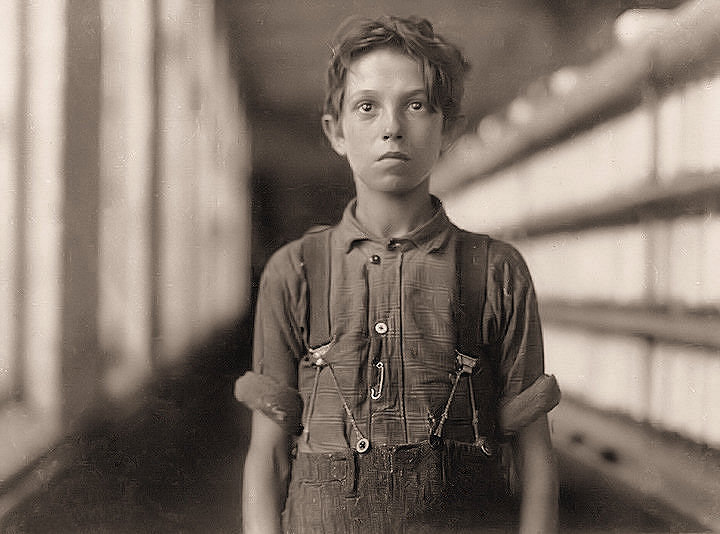
\includegraphics[height=203.5pt, width=5cm, keepaspectratio]{hine02}\hfill}
\vskip1pt
\vskip\baselineskip
\lipsum[1-10]\lipsum
\end{multicols}
\the\textheight\\
\the\paperheight

